\addsec{Introduction}
\markboth{Introduction}{}

Le cours de Conception de Circuits est structuré autour de l'étude du cas pratique d'un récepteur LIN. Les Travaux Dirigés (TD) sont consacrés à la méthodologie MCSE qui couvre la conception d'un système, de sa définition des contraintes à travers le cahier des charges, à ses spécifications initiales jusqu'à son implantation logique. La conception au niveau transistor, quant à elle, n'est pas traitée et fait l'objet d'un enseignement dédié dans le cours de Microélectronique.
\\

Les Travaux Pratiques (TP) viennent concrètement illustrer le flux de développement des circuits numériques présenté en TD. Ce rapport rend compte des travaux des sessions de TP qui consistaient en la description et validation complète du récepteur LIN.
\\

Il était dans un premier temps nécessaire de bien comprendre le cahier des charges. Puis, de descendre graduellement les couches d'abstraction pour arriver à la spécification et enfin la solution implémentée en TP.
La solution a été saisie sur le logiciel HDL Designer et testée avec ModelSim. La solution a pour objectif d’être implémentée sur FPGA. Le plan de ce rapport suit donc précisément cette progression méthodologique.

\newpage
\section{Rappel du cahier des charges}

Comme décrit plus haut, la forme que suit le cours de Conception de Circuit est celle d'une méthodologie classique de MCSE et plus particulièrement de MCCE ou Méthodologie de Conception de Circuits Electroniques. Cette méthodologie est une méthodologie descendante ou top-down qui se veut être un guide d'étape à suivre pour le concepteur afin de bien concevoir un circuit. Ce guide consiste en une succession d'étapes qui transforment une entrée (Spécification qui dérive du Cahier des Charges) en une sortie (la solution matérielle). Pour ce faire, une étape contient des outils qui permet au concepteur de visualiser les différents niveaux de précision de conception d'un circuit mais d'aussi de basculer d'un type de représentation (comportementale ou structurelle) à une autre.
Pour illustrer cette méthodologie, le diagramme en Y visible sur la \autoref{fig:diagram_y} est incontournable.

\begin{figure}[H]
    \centering
    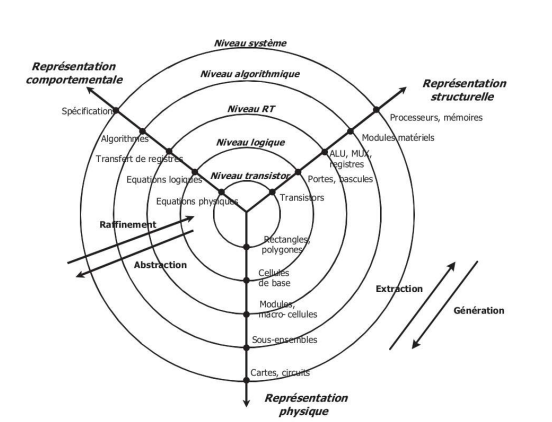
\includegraphics[width=0.8\linewidth]{figures/diagY.png}
    \caption{Diagramme en Y}
    \label{fig:diagram_y}
\end{figure}

La partie Représentation Physique du diagramme n'est pas vraiment traitée dans le cadre de ce cours. Ce diagramme donne la stratégie à suivre pour bien confectionner le LIN Receiver et celle-ci commence par les spécifications qui découlent elles-mêmes de l'élaboration d'un cahier des charges et de la définition des contraintes souhaitées pour ce système.

\subsection{Du Besoin à la Définition des contraintes}
\subsubsection{Qu'est-ce qu'un récepteur LIN ?}
L'étape de Définition des contraintes est le processus qui consiste à comprendre les besoins du client et à documenter ces besoins. L'accent est mis sur la compréhension du problème que le système doit résoudre, en se concentrant ainsi sur l'environnement dans lequel le système fonctionnera et non sur le système en lui-même.

Le Cahier Des Charges de ce projet a pour objectif final de concevoir un récepteur LIN ou Local Interconnect Network. Ce récepteur LIN doit communiquer avec un microprocesseur. Le récepteur à concevoir sera un périphérique du microprocesseur.

Avant de définir ce qu'est un récepteur LIN, il faut savoir ce qu'est le protocole de communication LIN, dont le récepteur fait partie.
Le LIN est un protocole de communication série complémentaire au bus CAN ou Controller Area Network. Ces deux protocoles sont très répandus dans l'industrie automobile mais pas pour les mêmes fonctions.
Le CAN est un standard de communication qui lui est conçu pour relier les unités de contrôle électroniques dans des applications temps réel exigeantes, comme la gestion moteur ou les airbags. Le CAN réagit vite et possède une grande fiabilité, ce qui en fait le protocole de communication privilégié pour les fonctions où la gestion du temps est critique. Le LIN quant à lui est conçu pour les applications moins critiques, où le coût prime sur les performances. 

\begin{figure}[H]
    \centering
    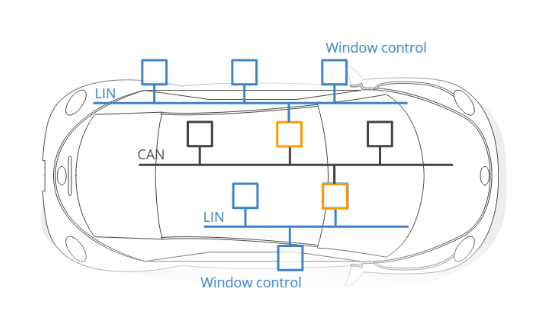
\includegraphics[width=0.7\linewidth]{figures/Exemple_LIN_voiture.png}
    \caption{Protocole CAN et LIN dans une voiture}
    \label{fig:can_lin_in_car}
\end{figure}

Ce système de communication est très utilisé dans les voitures pour commander des équipements simples comme les vitres, les essuie-glaces ou la climatisation. Un réseau LIN fonctionne avec un module principal (l'hôte) qui peut contrôler jusqu'à 16 modules secondaires (les clients).
Le récepteur LIN que nous devons concevoir fait partie intégrante des nœuds clients.

\begin{figure}[H]
    \centering
    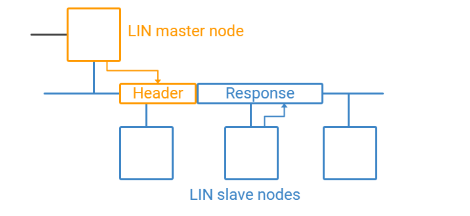
\includegraphics[width=0.7\linewidth]{figures/Architecture_bus_LIN.png}
    \caption{Architecture d'un bus LIN}
    \label{fig:archi_bus_lin}
\end{figure}

Le récepteur LIN surveille constamment le bus de communication et agit si un message lui est adressé. Chaque message envoyé par le nœud hôte contient un identifiant PID ou Protected IDentifier. Le récepteur doit donc reconnaître si le message lui est destiné et si tel est le cas récupérer le contenu du message. En clair, lorsque le récepteur LIN reconnaît un message de l'hôte qui lui est adressé, il le capture et le décode. Il transmet ensuite les instructions au microcontrôleur, le "cerveau" du module, qui exécute la commande (par exemple, "monter la vitre").

\subsubsection{Comment fonctionne un récepteur LIN ?}

Une trame de message sur un bus LIN est composée d'un header et d'une réponse/information. L'hôte transmet le header sur le bus. Celui-ci déclenche un client, qui envoie une réponse. La structure générale d'une trame LIN peut être illustrée comme suit :

\begin{figure}[H]
    \centering
    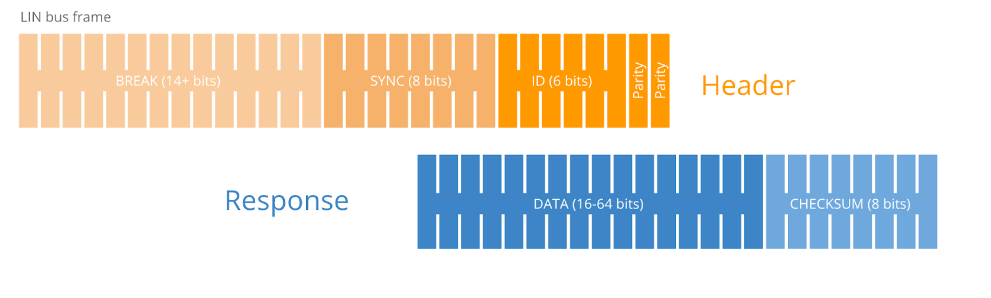
\includegraphics[width=0.9\linewidth]{figures/LIN_Format.png}
    \caption{Structure d'une trame LIN}
    \label{fig:struct_trame_lin}
\end{figure}

En vérité, le CDC demande un récepteur LIN avec des exigences spécifiques : celle d'un récepteur LIN limité. Ainsi le récepteur à concevoir n'aura qu'une vitesse de transmission de 19200 bit/s à recevoir et la trame à recevoir dans sa partie réponse sera amputée de sa partie Checksum Field. De plus, les bits de parité ne seront pas considérés dans la section Identifier Field.
Précisément, le circuit a concevoir est un circuit d'interfaçage qui devra être capable de comprendre et assimiler le protocole LIN et de communiquer avec le micro-processeur.

\subsubsection{Structure d'une trame LIN}

La trame LIN que le récepteur doit reconnaître puis répondre est composée de plusieurs parties distinctes qui assurent la synchronisation, l'identification et la transmission des données.

\begin{figure}[H]
    \centering
    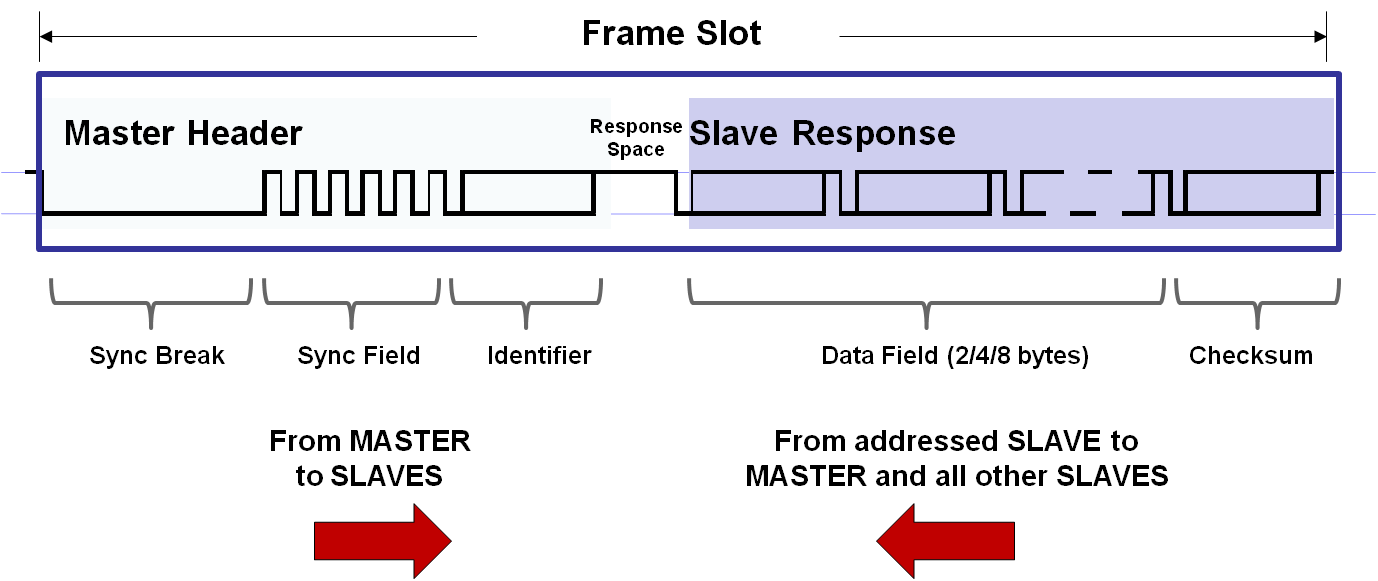
\includegraphics[width=0.9\linewidth]{figures/trame/frame-slot.png}
    \caption{Structure d'une trame LIN détaillée}
    \label{fig:detailled_lin_frame}
\end{figure}

\bigskip
\textbf{Synchronization Break}
\bigskip

Le Synchronization Break est une séquence de synchronisation composée d'au moins 13 bits à l'état bas (dominant) suivis d'au moins 1 bit à l'état haut (récessif). Cette impulsion distinctive sert de signal de début de trame, ce qui avertit tous les nœuds du bus qu'une transmission est imminente.

\begin{figure}[H]
    \centering
    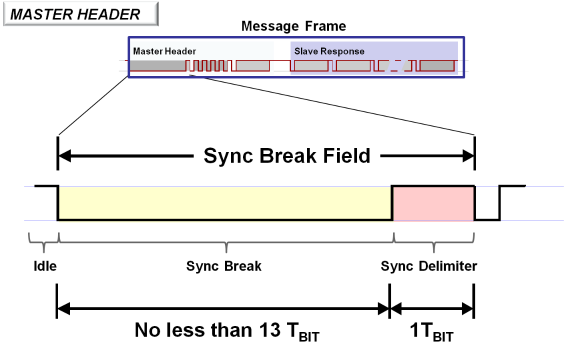
\includegraphics[width=0.7\linewidth]{figures/trame/master-header-sync-break.png}
    \caption{Détail de la partie Synchronization Break de la trame}
    \label{fig:synchro_break}
\end{figure}

\bigskip
\textbf{Synchronization Field}
\bigskip

Le Synchronization Field contient la valeur fixe 0x55 (soit 01010101 en binaire). Cette séquence régulière de 0 et de 1 permet aux nœuds clients de déterminer la vitesse de communication de l’hôte en mesurant le temps entre chaque changement d'état. Ils adaptent ainsi leur débit pour se synchroniser.

\begin{figure}[H]
    \centering
    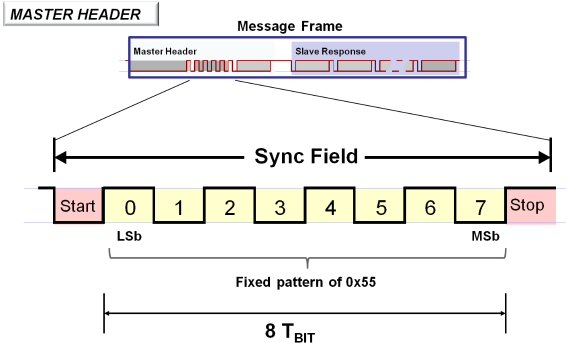
\includegraphics[width=0.7\linewidth]{figures/trame/master-header-sync-field.png}
    \caption{Détail de la partie Synchronization Field de la trame}
    \label{fig:synchro_field}
\end{figure}

\bigskip
\textbf{Identifier Field}
\bigskip

L’Identifier Field est codé sur 6 bits, auxquels s'ajoutent 2 bits de parité que l’on a choisi d’ignorer d’après le CDC. L’Identifier Field identifie le message et détermine quel nœud client doit y réagir. Les clients peuvent ensuite :

\begin{enumerate}
    \item Ignorer la transmission de données qui suit.
    \item Écouter les données transmises par un autre nœud.
    \item Publier des données en réponse au header.
\end{enumerate}

En général, un seul client est interrogé à la fois. 

\begin{figure}[H]
    \centering
    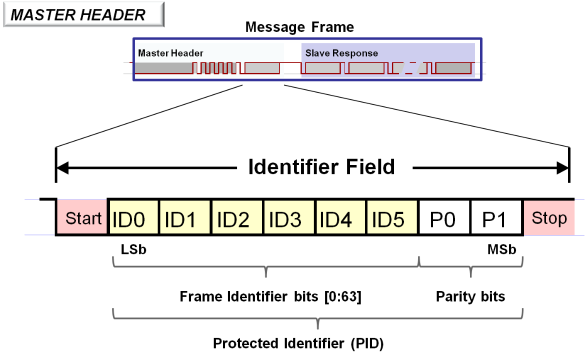
\includegraphics[width=0.7\linewidth]{figures/trame/master-header-identifier-field.png}
    \caption{Détail de la partie Identifier Field de la trame}
    \label{fig:id_field}
\end{figure}

\bigskip
\textbf{Data Field}
\bigskip
Les informations sont transmises dans les Data Field, chacun contenant un octet de donnée. Une trame peut contenir 2,4 ou 8 Data Field. Le nombre de Data Field est codé par les bits 4 et 5 de l'Identifier Field. Le nombre de Data Field est ensuite déterminé par un décodage.
Dans le cadre d'une écriture, les Data Fields sont envoyés par l'hôte. Dans le cadre d'une lecture, les Data Fields sont envoyés par le client, comme réponse à la demande de l’hôte.


\begin{figure}[H]
    \centering
    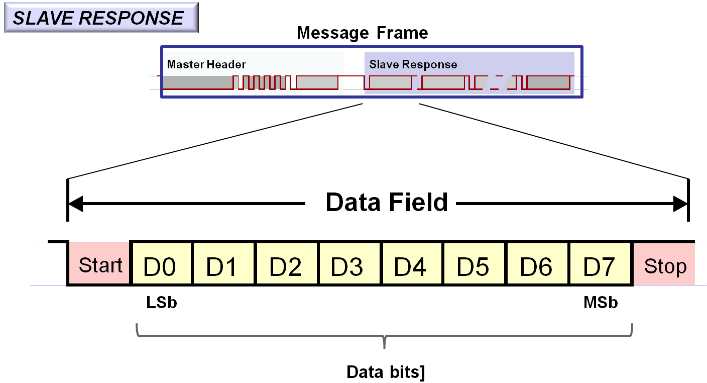
\includegraphics[width=0.7\linewidth]{figures/trame/slave-response-data-field.png}
    \caption{Détail de la partie Data Field de la trame}
    \label{fig:data_field}
\end{figure}

\subsubsection{Position du circuit à designer et interaction avec son environnement}

Avant de délimiter les entrées et sorties du système, il est essentiel de définir son contexte opérationnel et les acteurs externes avec lesquels il interagit.
Finalement, les entités en interaction avec le système à concevoir sont les suivantes (une interaction étant définie comme un échange provoquant une réaction) :
    \begin{itemize}
    \item L'émetteur LIN (LIN Transmitter): Il délivre les données série à recevoir. La communication est régie par le protocole LIN, qui impose son format de trame et son débit binaire comme indiqué précédemment.
    \item Le microprocesseur : Ce système dialogue avec le circuit conçu. Il a pour rôles principaux : de lire les informations provenant du circuit, telles que son état interne (status) et les données reçues et validées, mais aussi d'écrire des informations de configuration ou de commande, comme une adresse de sélection \texttt{SelAdr}.
\end{itemize}

\subsubsection{Délimitation des entrées sorties}

L'objectif de cette partie est de définir les relations entre le système et ses entités. Le schéma des entrées sorties est visible sur la \autoref{fig:input_output_system_schema}.

\begin{figure}[H]
    \centering
    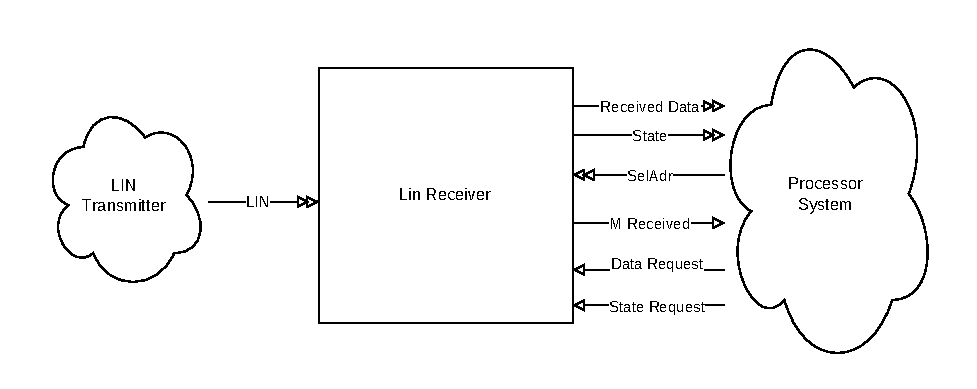
\includegraphics[width=0.9\linewidth]{figures/input_output_system_schema.pdf}
    \caption{Entrées et sorties du système par rapport à son environnement}
    \label{fig:input_output_system_schema}
\end{figure}
Définitions des relations :

\paragraph{Relation LIN}
\begin{itemize}
    \item DefLin = (active, inactive) = (0,1)
    \item Relation permanente
\end{itemize}

\paragraph{Relation Received Data}
\begin{itemize}
    \item DefByte = array[0...7] of DefBit
    \item Relation permanente
\end{itemize}

\paragraph{Relation M Received, Data Request et State Request}
\begin{itemize}
    \item Relation immédiate
    \item aucunes données lié à ces relations.
\end{itemize}

\paragraph{Relation SelAdr}
\begin{itemize}
    \item DefByte = array[0...7] of DefBit
    \item Relation permanente
\end{itemize}

\paragraph{Relation State}
\begin{itemize}
    \item Type de données : 
    \begin{itemize}
        \item DefByte = array [0...7] of DefBit
        \item DefState = 
        \begin{itemize}
            \item Message complet : DefByte + 
            \item Nombre de Bytes : DefNbBytes +
            \item Error State : DefError + 
            \item Error Start : DefError + 
            \item Error Stop : DefError + 
            \item Error Synchronization : DefError
        \end{itemize}
        
    \end{itemize}

    \item Relation permanente
\end{itemize}


\section{Spécification}
\subsection{Spécification Fonctionnel}
\label{section:specification_fonctionnel}
L'objectif est de capturer l'évolution attendue du circuit du point de vue des entités. Les évolutions seront décrites par des automates. L'objectif est de décrire les possibles états du circuit.

\subsubsection{Évolution attendue du point de vue du transmetteur LIN}
L'évolution attendue du point de vue du transmetteur LIN est détaillée avec le plus haut niveau d'abstraction sur le schéma  \autoref{fig:func_spec_lin_transmitter_perspective}.

\begin{figure}[H]
    \centering
    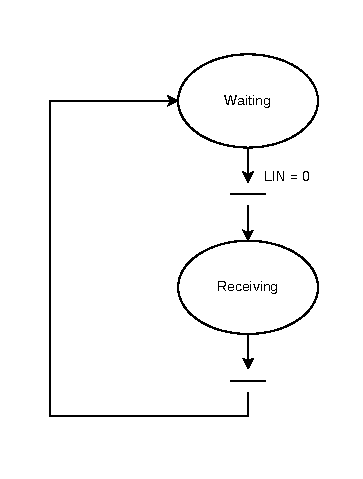
\includegraphics[width=0.4\linewidth]{figures/spec/func_spec_lin_transmitter_perspective.pdf}
    \caption{Automate de l'évolution attendue du point de vue du transmetteur LIN}
    \label{fig:func_spec_lin_transmitter_perspective}
\end{figure}


Une représentation plus en détail est présentée sur la \autoref{fig:func_spec_lin_transmitter_perspective_finer_grain}. Sur cet automate plus détaillé, les état \textit{Synchro break Reception} et \textit{Synchro field Reception} sont détaillés et explicités sur les \autoref{fig:func_spec_lin_transmitter_perspective_finer_grain_synchrobreak} et \autoref{fig:func_spec_lin_transmitter_perspective_finer_grain_synchrofield} respectivement.

L'automate détaillé suit simplement la spécification d'une trame LIN et récupère donc les différents type d'informations : \textit{Synchro break}, \textit{Synchro field}, \textit{Identifier field}, \textit{Data field} et \textit{Checksum field}, de manière séquentielle.\\

Le raffinement de \textit{Synchro break Reception} (\autoref{fig:func_spec_lin_transmitter_perspective_finer_grain_synchrobreak}) met en avant la nécessité de tester la valeur de LIN à l’état bas pendant au moins 13 intervalles de temps (noté ici Tbits) puis au minimum 1 intervalle de temps à l'état haut.
Tbits dépend de la fréquence de communication utilisée entre le transmetteur et le récepteur LIN.\\

Le raffinement de \textit{Synchro field Reception} (\autoref{fig:func_spec_lin_transmitter_perspective_finer_grain_synchrofield}) met en avant la lecture des 8 bits tous les Tbits. La lecture en milieu de bit est réalisée par la transition entre l'état \texttt{Start} et \texttt{Data Bits} qui a lieu après un temps de $\frac{Tbits}{2}$. Cela permet de réaliser tous les échantillonnages suivants en milieu de bit.
La lecture du bit est indiquée par le stockage dans RecByte.\\

\begin{figure}[H]
    \centering
    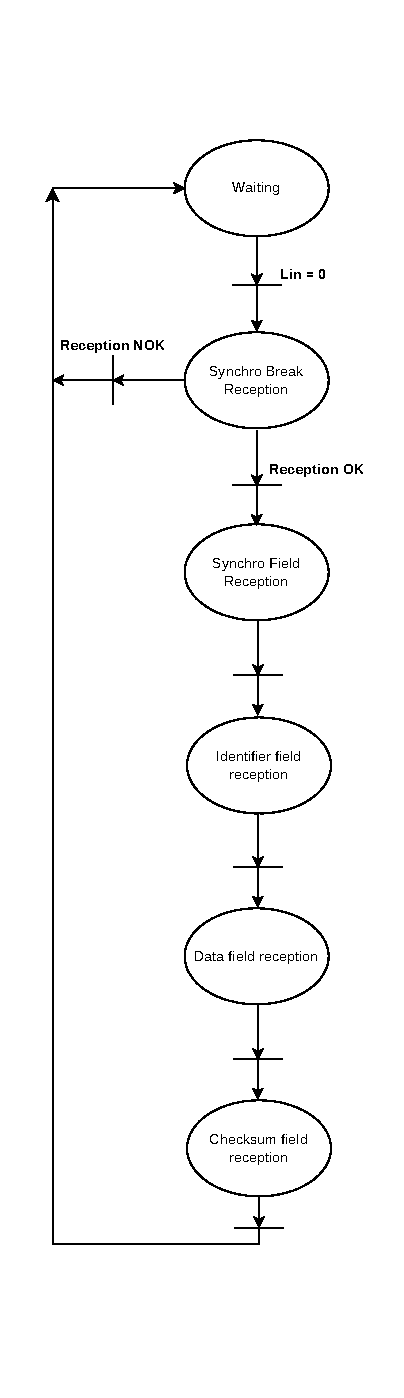
\includegraphics[width=0.4\linewidth]{figures//spec/func_spec_lin_transmitter_perspective_finer_grain.pdf}
    \caption{Automate détaillé de l'évolution attendue du point de vue du transmetteur LIN}
    \label{fig:func_spec_lin_transmitter_perspective_finer_grain}
\end{figure}

\begin{figure}[H]
    \centering
    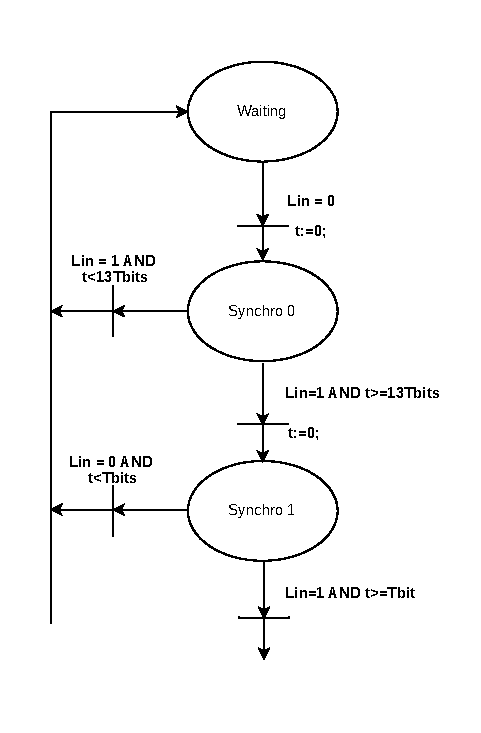
\includegraphics[width=0.7\linewidth]{figures/spec/func_spec_lin_transmitter_perspective_finer_grain_synchrobreak.pdf}
    \caption{Automate détaillé de l'évolution de \textit{Synchro break Reception} attendue du point de vue du transmetteur LIN}
    \label{fig:func_spec_lin_transmitter_perspective_finer_grain_synchrobreak}
\end{figure}

\begin{figure}[H]
    \centering
    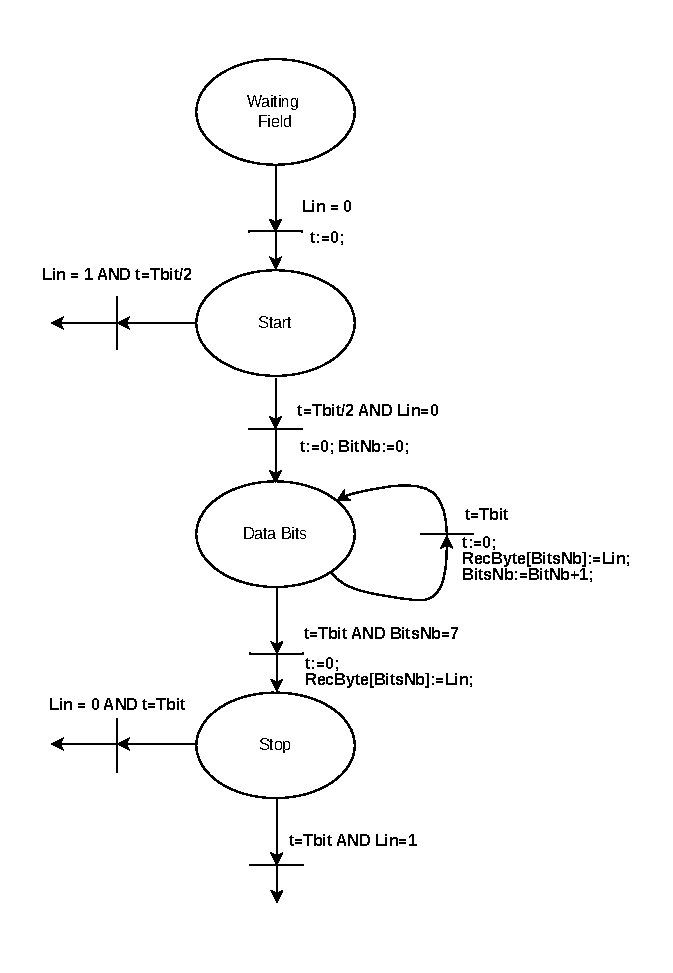
\includegraphics[width=0.7\linewidth]{figures/spec/func_spec_lin_transmitter_perspective_finer_grain_synchrofield.pdf}
    \caption{Automate détaillé de l'évolution de \textit{Synchro field Reception} attendue du point de vue du transmetteur LIN}
    \label{fig:func_spec_lin_transmitter_perspective_finer_grain_synchrofield}
\end{figure}


\subsubsection{Évolution attendue du point de vue du processeur}
L'évolution attendue du point de vue du processeur est détaillée avec le sur le schéma \autoref{fig:func_spec_processor_perspective}.

\begin{figure}[H]
    \centering
    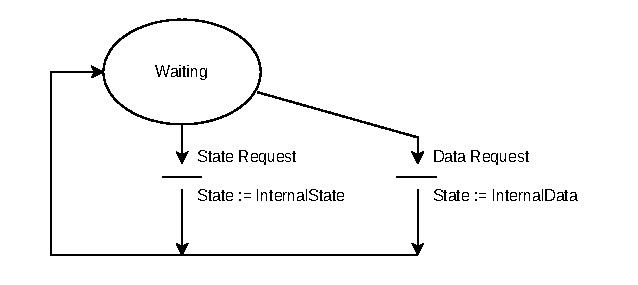
\includegraphics[width=0.7\linewidth]{figures/spec/func_spec_processor_perspective.pdf}
    \caption{Automate de l'évolution attendue du point de vue du processeur}
    \label{fig:func_spec_processor_perspective}
\end{figure}

\subsection{Spécification Opérationnel}
Pour ce système, les spécifications opérationnelles sont les suivantes.

L'utilisation d'une mémoire FIFO pour stocker les données est demandée.
Cela permet de ne pas gérer les adresses des données à stocker.

Le test de la valeur du signal LIN reçu doit être réalisé au milieu des bits. Il est donc nécessaire d'avoir une fréquence d'échantillonnage du signal LIN assez élevée pour permettre une mesure au milieu du bit.

\subsection{Spécification Technologique}
La solution conçue sera implémentée sur un FPGA Xilinx Artix 7.

\subsubsection{Interface avec le microprocesseur}
Au niveau de l’interface avec le microprocesseur, les signaux sont imposés. Ils sont visibles sur la \autoref{fig:circuit_to_micro} et détaillés ci-après. En plus des signaux de contrôle, le récepteur LIN à concevoir devra notifier le microprocesseur via un signal de fin de réception (\texttt{MReceived}) lorsqu’une trame à sa destination a été correctement reçue. 

\begin{figure}[H]
    \centering
    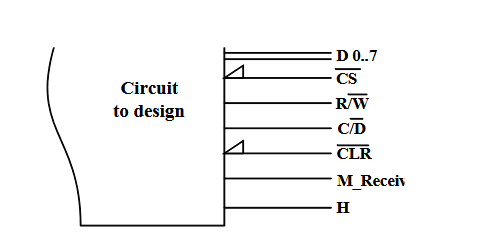
\includegraphics[width=0.7\linewidth]{figures/spec/interface_micro_to_design.png}
    \caption{Interface entre le circuit et le microprocesseur}
    \label{fig:circuit_to_micro}
\end{figure}

Voici les différents signaux que vont échanger le circuit et le microprocesseur : 

\begin{itemize}
    \item D07 =  Bus de données bidirectionnel de 8 bits.
    \item $\overline{CS}$ = Signal de sélection de circuit.
    \item $R/\overline{W}$ = Contrôle la direction du transfert : Lecture (High) ou Écriture (Low).
    \item $C/\overline{D}$ = Signal de commande détermine si le bus de données transporte une donnée (niveau bas) ou une instruction/une adresse (niveau haut).
    \item $\overline{CLR}$ = Signal de réinitialisation du circuit (reset) actif niveau bas.
    \item $M\_Receive$ = Signal de fin de réception.
    \item $H$ = Signal d'horloge.\\
    
\end{itemize}

En plus des signaux, le microprocesseur impose des contraintes temporelles. Celles-ci sont visibles sur la \autoref{fig:interface_micro_temporal_constraints}. 
Ces contraintes ne sont pas testées dans le cadre de ce cours.


\begin{figure}[H]
    \centering
    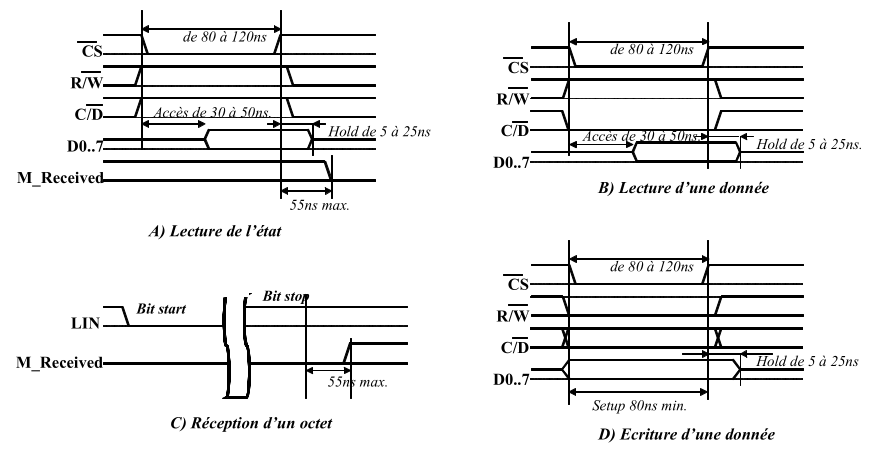
\includegraphics[width=0.95\linewidth]{figures/spec/interface_micro_temporal_constraints.png}
    \caption{Contraintes temporelles imposées par le microprocesseur}
    \label{fig:interface_micro_temporal_constraints}
\end{figure}


L'ensemble de la spécification est maintenant défini. Il est donc possible de détailler la structure fonctionnelle mise en place pour ce système.

\section{Description et Justification de la structure fonctionnelle}
Les deux points de vue du système détaillés dans la \autoref{section:specification_fonctionnel} permettent de définir deux blocs internes au système : \textit{Lin Reception} et \textit{Processor Interface}.

\begin{comment}
Il est aussi bon usage de définir une interface pour découpler le fonctionnement du récepteur en lui-même de la communication avec le processeur. L'objectif de l'interface est de faire la liaison entre les trames reçues et les signaux de contrôle imposés par le cahier des charges.\\
\end{comment}

La structure fonctionnelle est exprimée au niveau algorithmique du diagramme en Y (\autoref{fig:diagram_y}). Au niveau algorithmique, les blocs peuvent être dépendants d'une horloge de référence. Le bloc \textit{Lin Reception} possède son horloge de référence définie par le bloc \textit{Clock Generation}. 

Il est naturel que le bloc \textit{Lin Reception} indique au bloc \textit{Processor Interface} son état interne et les données internes, pour que l'interface puisse indiquer les bonnes valeurs au processeur.

L'ensemble de ces blocs et liaison sont schématisé sur la \autoref{fig:functionnal_schema}.

\begin{figure}[H]
    \centering
    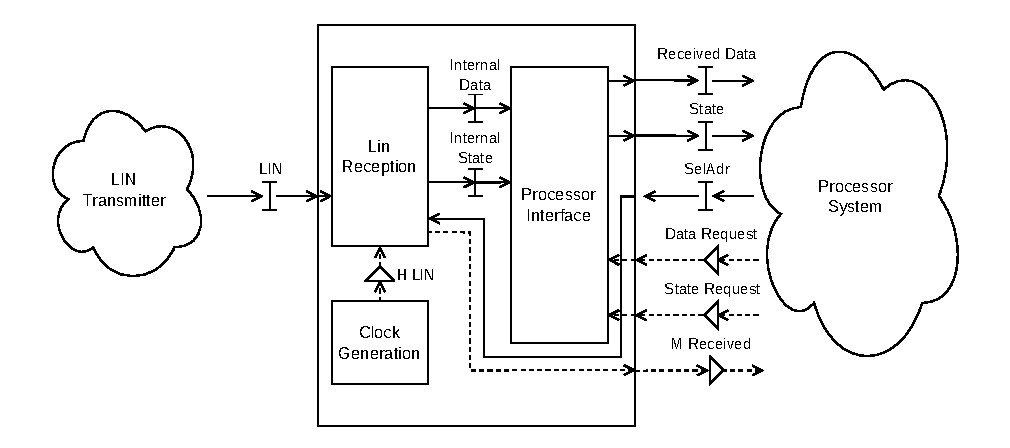
\includegraphics[width=1\linewidth]{figures/functional/functionnal_schema.pdf}
    \caption{Schéma de la structure fonctionnelle}
    \label{fig:functionnal_schema}
\end{figure}


\subsection{Comportement du bloc \textit{Lin Reception}}
Le comportement du bloc est un raffinement de l'évolution du point de vue du transmetteur Lin décrit en \autoref{fig:func_spec_lin_transmitter_perspective_finer_grain}.
En particulier, les dépendances au temps sont devenues des dépendances à un compteur. N est ainsi défini comme le rapport entre la période de la vitesse de la communication LIN et la période de l'horloge \textit{Clock Generation}.\\

\begin{equation}
    N = \frac{T_{bits}}{T_{H LIN}}
    \label{eq:N}
\end{equation}

Le comportement détaillé de \textit{Synchro break Reception} et \textit{Synchro field Reception} sont visibles sur les \autoref{fig:func_lin_transmitter_perspective_finer_grain_synchrobreak} et \autoref{fig:func_lin_transmitter_perspective_finer_grain_synchrofield} respectivement.
Sur l'automate de \textit{Synchro field Reception}, lors de la transition entre Stop Bit Reception et Waiting Identifier Field, RecByte est stocké dans l'état ReceiveByte. De plus, le nombre d'octets stockés dans la FIFO est incrémenté de 1.
Sur la \autoref{fig:func_spec_lin_transmitter_perspective_finer_grain}, \texttt{Internal Data} devient donc \texttt{ReceiveByte}.



\begin{figure}[H]
    \centering
    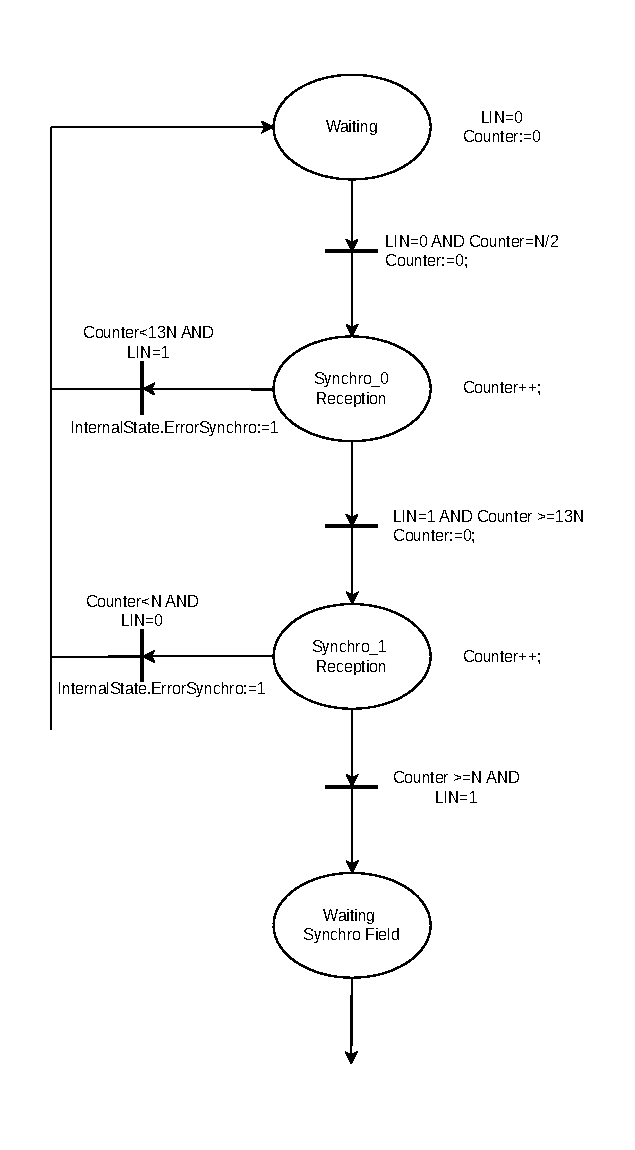
\includegraphics[width=0.7\linewidth]{figures/functional/func_lin_transmitter_perspective_finer_grain_synchrobreak.pdf}
    \caption{Automate détaillé du comportement \textit{Synchro break Reception}}
    \label{fig:func_lin_transmitter_perspective_finer_grain_synchrobreak}
\end{figure}

\begin{figure}[H]
    \centering
    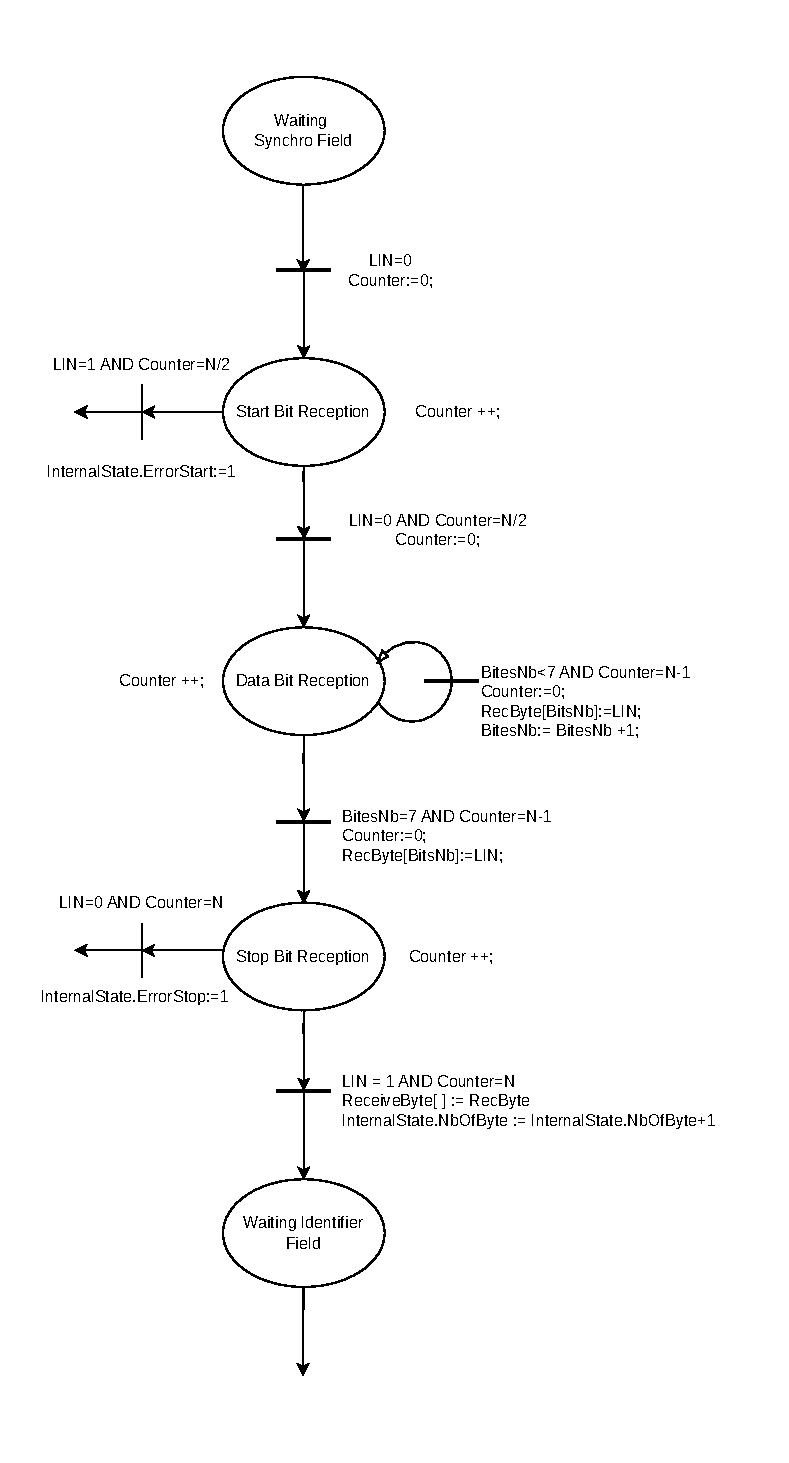
\includegraphics[width=0.7\linewidth]{figures/functional/func_lin_transmitter_perspective_finer_grain_synchrofield.pdf}
    \caption{Automate détaillé du comportement \textit{Synchro field Reception}}
    \label{fig:func_lin_transmitter_perspective_finer_grain_synchrofield}
\end{figure}

\subsection{Comportement du bloc \textit{Processor Interface}}
Le comportement du bloc \textit{Processor Interface} est un raffinement  de l'évolution du point de vue du processeur décrit en \autoref{fig:func_spec_processor_perspective}. 
Le comportement est décrit dans l'automate présent \autoref{fig:func_processor_interface}.

Lors d'une demande d'état, l'état courant est renvoyé puis est chaque composante est reset à sa valeur par défaut.
Lors d'une demande de donnée, le nombre d'octets stocké en interne dans la FIFO est réduit de 1.

\begin{figure}[H]
    \centering
    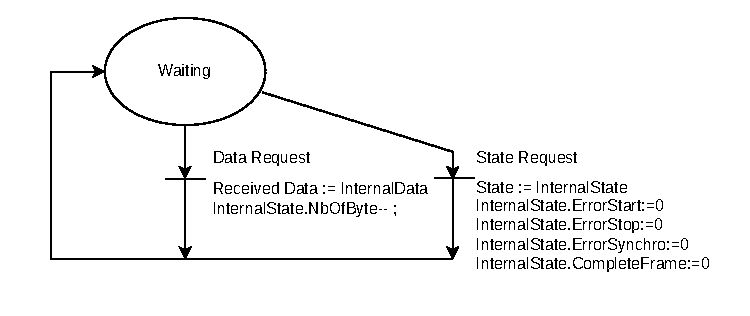
\includegraphics[width=0.75\linewidth]{figures//functional/func_processor_interface.pdf}
    \caption{Automate du comportement du bloc \textit{Processor Interface} }
    \label{fig:func_processor_interface}
\end{figure}


\section {Description et Justification de la solution architecturale}
Pour arriver à la solution architecturale, il faut passer du niveau Algorithme au niveau Transfert de Registre.

\subsection{Interface physique avec le processeur}
La première étape est l'introduction d'interfaces de communication, en particulier l'interface physique de communication avec le processeur. C'est cette interface qui va gérer tout les signaux indiqués dans le cahier des charges : $D07$, $CLR$, $CS$, $RW$, $CD$ et $H_{proc}$.

Le comportement de cette interface implémente les différents modes du cahier des charges en fonction de l'état des signaux d'entrée.
Le comportement est visible sur la \autoref{fig:archi_behavior_physical_interface}.

\begin{figure}[H]
    \centering
    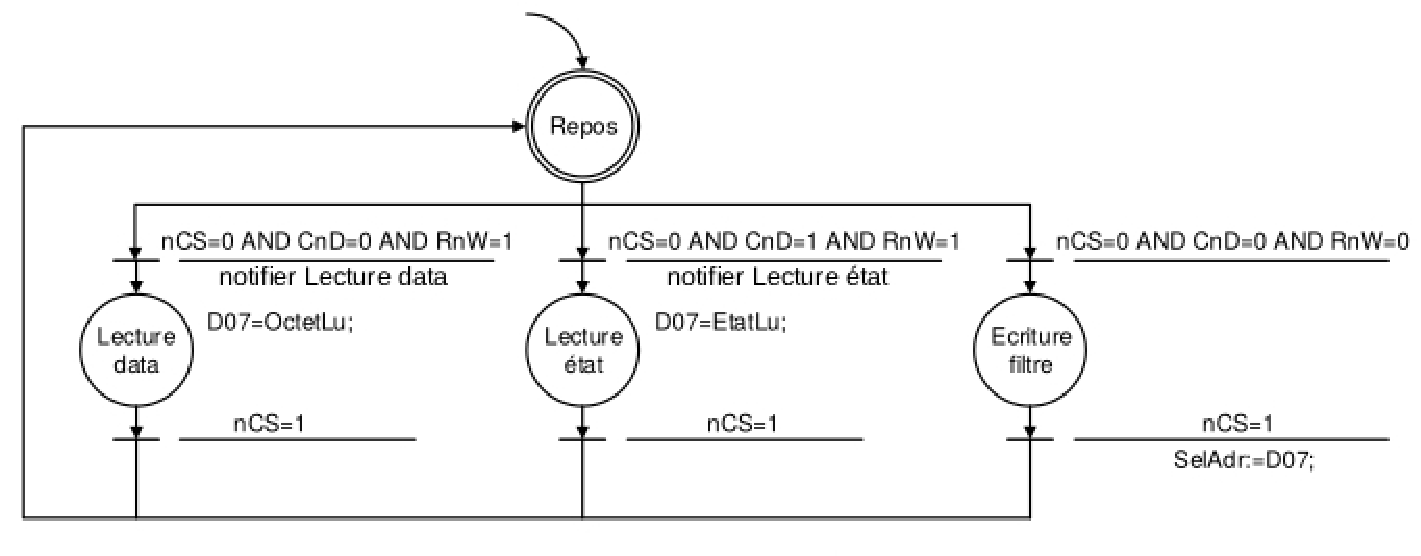
\includegraphics[width=0.75\linewidth]{figures/archi/archi_behavior_physical_interface.pdf}
    \caption{Comportement de l'interface physique de communication avec le processeur}
    \label{fig:archi_behavior_physical_interface}
\end{figure}

Il est cependant courant de fusionner le comportement de l'interface processeur décrit précédemment avec l'interface physique. Il en résulte une interface processeur V2. 

Un point important à remarquer est que l'interface processeur V2 reçoit maintenant l'adresse de filtre SelAdr. Il est donc nécessaire de la transmettre au bloc \textit{Lin Reception}. 
Le schéma visible en \autoref{fig:archi_circuit_structure_v1} permet d'apercevoir la première étape de raffinement. La donnée SelAdr est transmise de \textit{Processor Interface V2} vers \textit{Lin Reception}.\\

\begin{figure}[H]
    \centering
    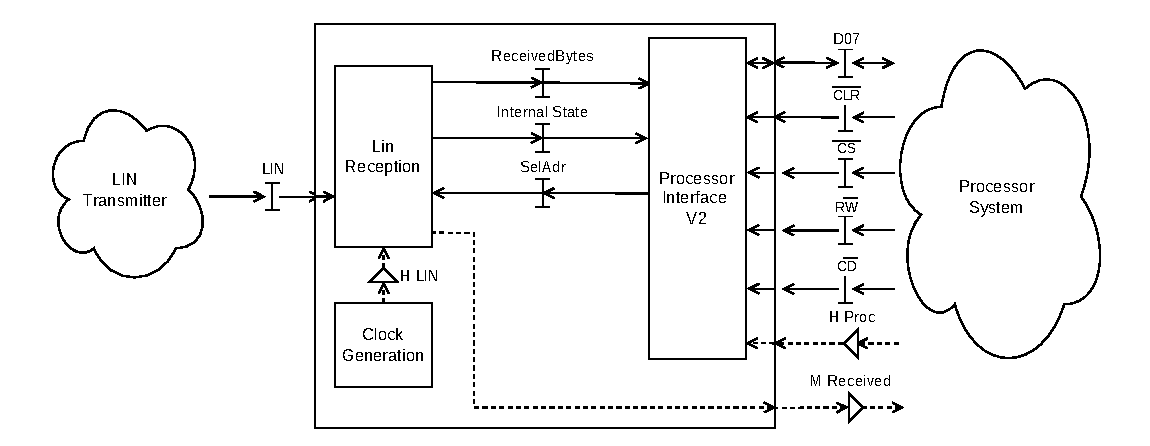
\includegraphics[width=1\linewidth]{figures/archi/archi_circuit_structure_v1.pdf}
    \caption{Structure du circuit avec le bloc \textit{Processor Interface V2}}
    \label{fig:archi_circuit_structure_v1}
\end{figure}

Il est aussi question de simplifier les domaines temporels, en utilisant une seule horloge pour tous les blocs du circuit. 
Le Lin Reception peut fonctionner à une fréquence très inférieure au processeur, mais utiliser une seule horloge permet de rendre le système plus simple.
Le générateur d'horloge ne sera donc pas utilisé et le ratio N défini précédemment sera utilisé dans le bloc Lin Reception.
Tout le système sera synchrone à l'horloge $H_{proc}$.


\subsection{Raffinement de ReceivedBytes}

Le cahier des charges impose ici l'utilisation d'une mémoire FIFO pour stocker les octets reçus par le récepteur LIN.
Une FIFO possède les signaux suivants : 
\begin{itemize}
    \item WENA : Write Enable
    \item RENA : Read Enable
    \item H : Clock
    \item Din : Data in
    \item Dout : Data out\\
\end{itemize}

Le signal ReceivedBytes devient donc le bloc détaillé dans la \autoref{fig:receivedBytes}.


\begin{figure}[H]
    \centering
    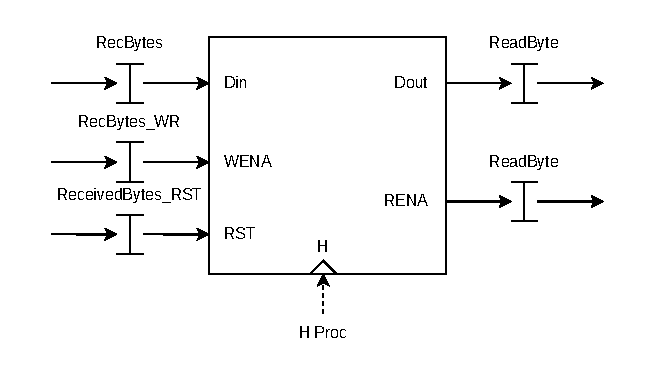
\includegraphics[width=0.6\linewidth]{figures//archi/receivedBytes.pdf}
    \caption{Bloc Received Byte FIFO obtenu après raffinement}
    \label{fig:receivedBytes}
\end{figure}

\subsection{Raffinement Internal State}

Internal State permet la transmission des informations suivantes :
\begin{itemize}
    \item CompleteFrame
    \item NbBytes
    \item ErrorStart
    \item ErrorStop
    \item ErrorSynchro
\end{itemize}
Ces informations doivent être gardées en mémoire provisoirement pour permettre le dialogue asynchrone entre les deux blocs : Lin Reception et Processor Interface. La mémoire sert de buffer.
Les 3 erreurs et CompleteFrame sont implémentées via 4 bascules RS. Le schéma de la bascule CompleteFrame est visible sur la \autoref{fig:CompleteFrameRS}, et est similaire pour les 3 erreurs.

\begin{figure}[H]
    \centering
    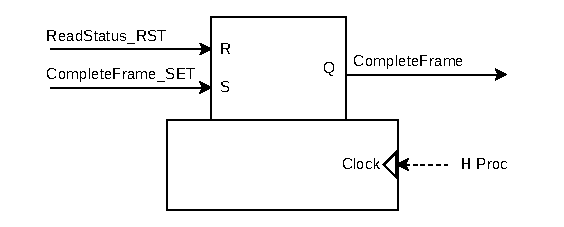
\includegraphics[width=0.6\linewidth]{figures//archi/CompleteFrameRS.pdf}
    \caption{Bascule RS pour synchroniser les signaux d'états}
    \label{fig:CompleteFrameRS}
\end{figure}


L'utilisation de bascule RS permet le reset avec le signal \texttt{ReadStatus\_RST} et de set la valeur avec \texttt{CompleteFrame\_SET}, \texttt{ErrorStart\_SET}, \texttt{ErrorStop\_SET} ou \texttt{ErrorSynchro\_SET}. \\


L'information NbBytes est implémentée par un compteur/décompteur sur 4 bits, dont le schéma est visible sur la \autoref{fig:NbBytesCounter}.

\begin{figure}[H]
    \centering
    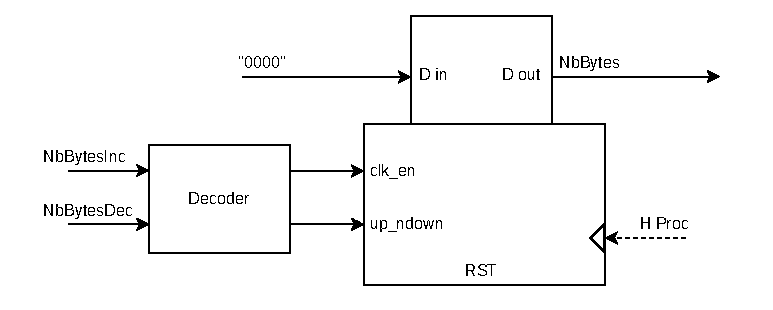
\includegraphics[width=0.75\linewidth]{figures//archi/NbBytesCounter.pdf}
    \caption{Schéma du raffinement de NbBytes en compteur/décompteur}
    \label{fig:NbBytesCounter}
\end{figure}


Le décodeur présent permet de contrôler le compteur/décompteur avec deux signaux : \texttt{NbByteInc} et \texttt{NbByteDec}.
La table de vérité du décodeur est présentée dans le \autoref{tab:truth_table_decoder}.

\begin{table}[H]
    \centering
    \begin{tabular}{cc||cc}
        NbByteInc & NbByteDec & $clk_{en}$ & $up/\overline{down}$\\
        \hline
        0 & 0 & 0 & 0\\
        0 & 1 & 1 & 0\\
        1 & 0 & 1 & 1\\
        1 & 1 & 0 & 0\\
    \end{tabular}
    \caption{Table de vérité du décodeur}
    \label{tab:truth_table_decoder}
\end{table}

Internal State est donc un bloc composé des bascules RS et du compteur/décompteur détaillé précédemment. L’ensemble du circuit est visible par la suite sur la \autoref{fig:archi_circuit_structure_v2}.

\subsection{Raffinement SelAdr}

L'information SelAdr doit être bufferisée et peut être implémentée par 8 bascules D. Le schéma de cette implémentation est visible sur la \autoref{fig:selAdr}.

\begin{figure}[H]
    \centering
    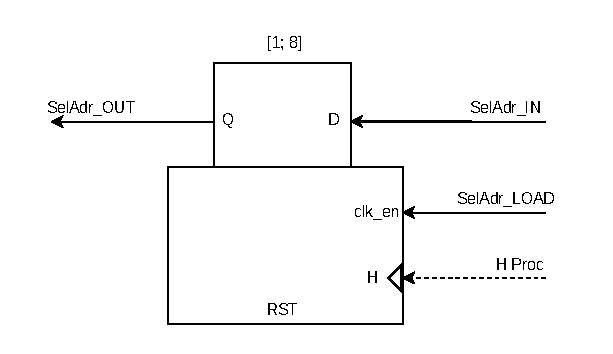
\includegraphics[width=0.75\linewidth]{figures//archi/selAdr.pdf}
    \caption{Raffinement de SelAdr}
    \label{fig:selAdr}
\end{figure}


\subsection{Description du schéma bloc raffiné}

L'ensemble des raffinements permet d'arriver au schéma présenté en \autoref{fig:archi_circuit_structure_v2}.

Cependant, l'implémentation sera simplifiée encore une fois.
La synchronisation de \texttt{SelAdr} via un buffeur sera réalisé dans Processor Interface V2.
\texttt{M\_Received} va devenir une variable partagée et vaut exactement \texttt{ReadStatus.CompleteFrame}.
Avec ces changements, la structure finale du récepteur LIN est visible sur la \autoref{fig:archi_circuit_structure_v3}.

Sur les deux schémas, le signal de reset est implicite pour des questions de lisibilité. L'ensemble des blocs sont reliés à $\overline{CLR}$.
De même sur la figure \autoref{fig:archi_circuit_structure_v3}, les blocs Received Bytes et Internal State sont aussi reliés à l'horloge H de manière implicite.

\begin{figure}[H]
    \centering
    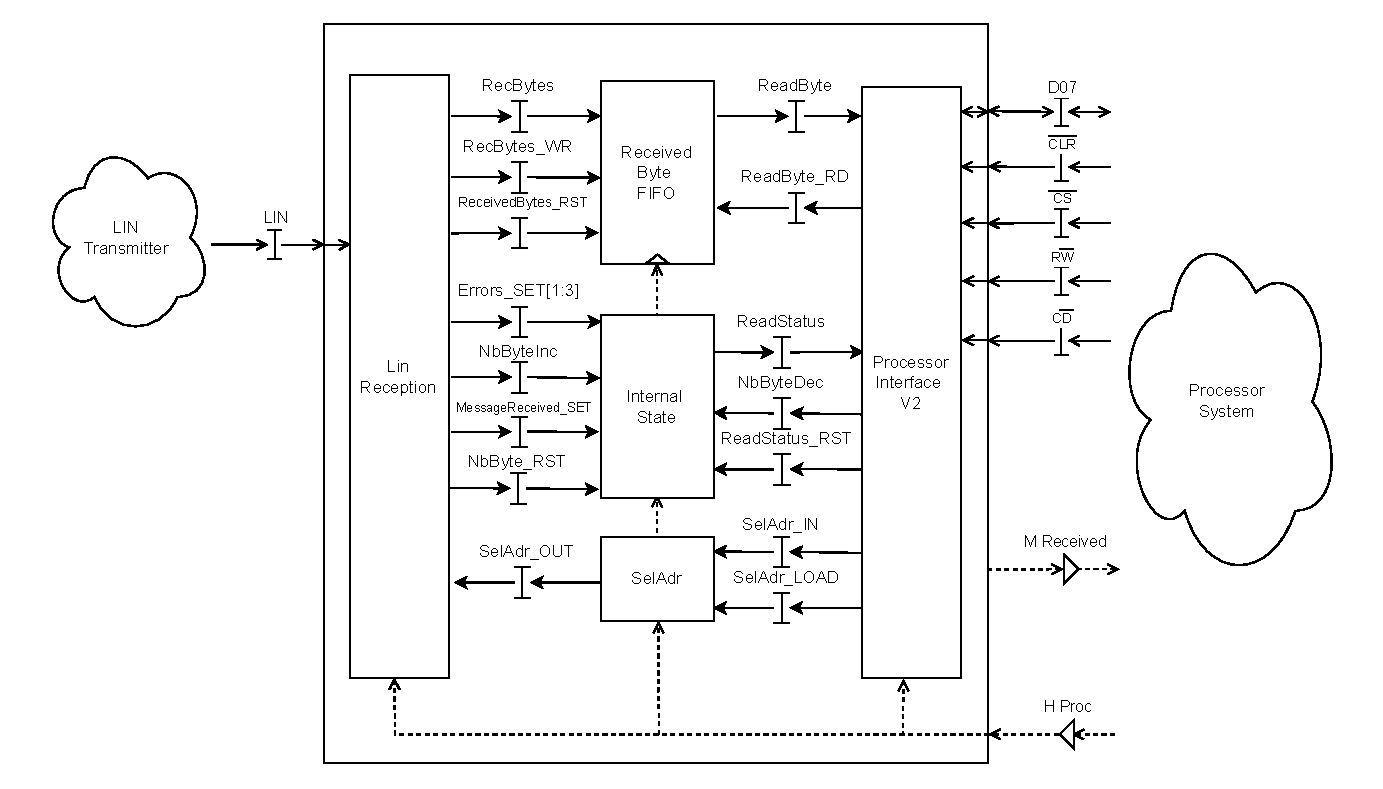
\includegraphics[width=1\linewidth]{figures/archi/archi_circuit_structure_v2.pdf}
    \caption{Description structurelle du récepteur LIN au niveau Transfert de Registre}
    \label{fig:archi_circuit_structure_v2}
\end{figure}


\begin{figure}[H]
    \centering
    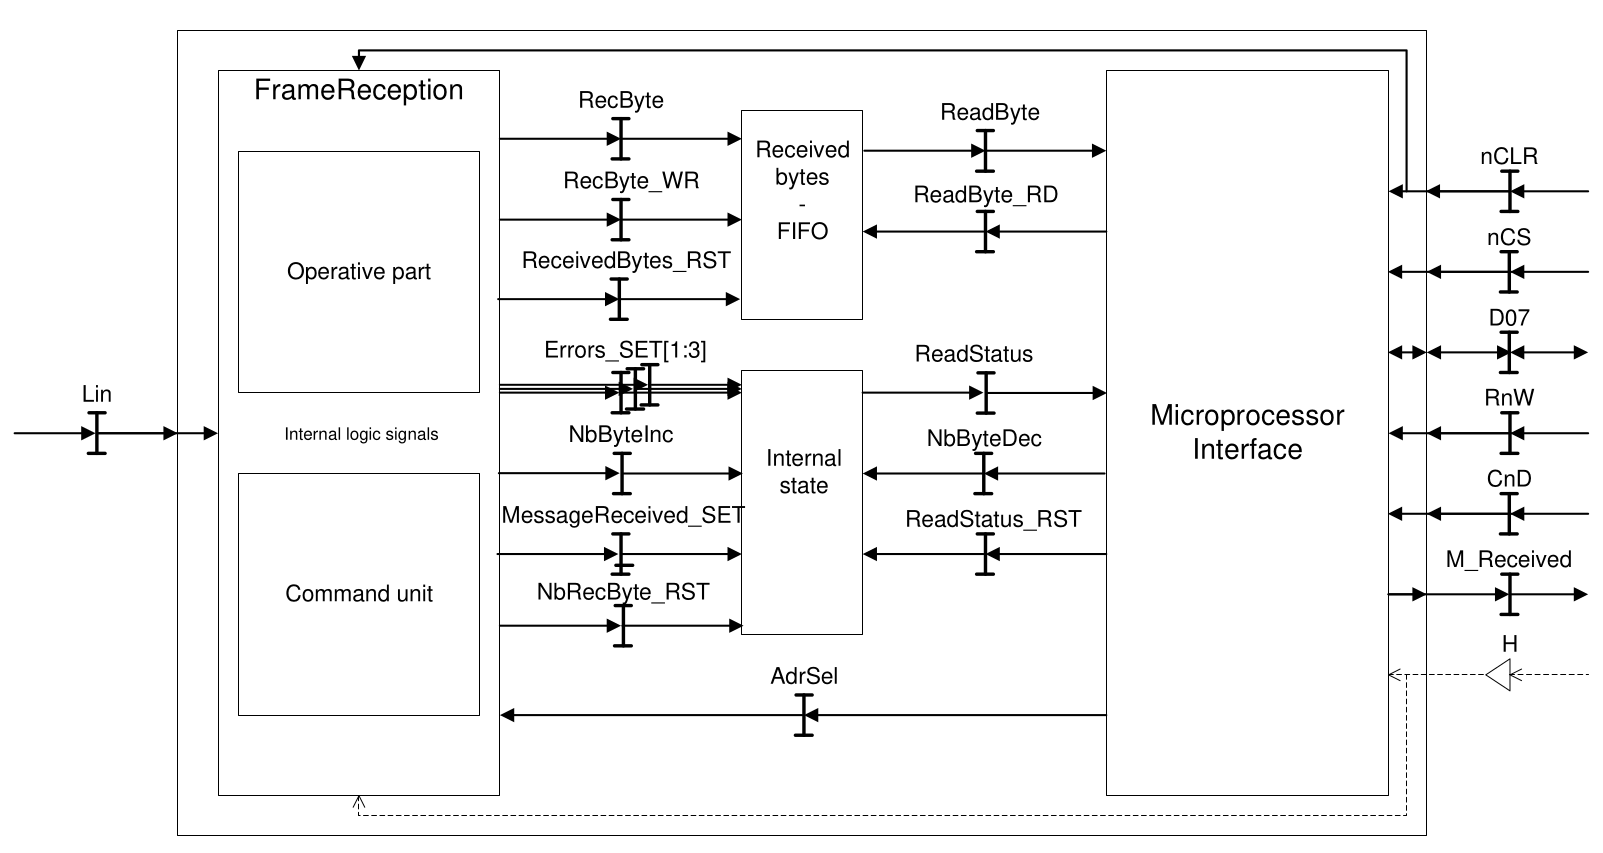
\includegraphics[width=1\linewidth]{figures/archi/archi_circuit_structure_v3.png}
    \caption{Description structurelle finale du récepteur LIN au niveau Transfert de Registre}
    \label{fig:archi_circuit_structure_v3}
\end{figure}

\subsection{Comportement de Processor Interface}

Avec le raffinement terminé, il est maintenant possible de d'avoir le comportement final du bloc Processor Interface. C'est un raffinement du comportement déjà présenté en \autoref{fig:archi_behavior_physical_interface}.
Ce comportement final est décrit dans la \autoref{fig:behavior_processor_interface}

\begin{figure}[H]
    \centering
    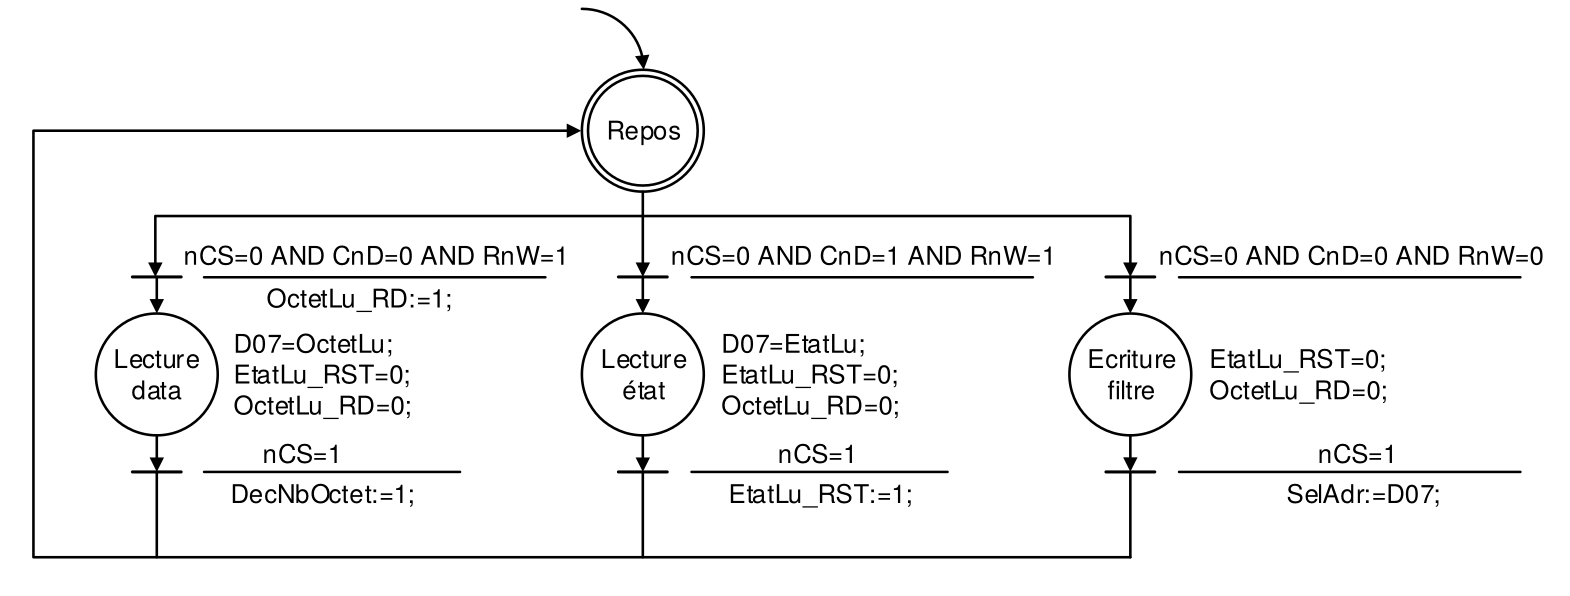
\includegraphics[width=1\linewidth]{figures/archi/behavior_processor_interface.png}
    \caption{Comportement final de l’interface de communication avec le processeur}
    \label{fig:behavior_processor_interface}
\end{figure}

\subsection{Comportement de Lin Receiver}
Lors du passage au niveau transfert de registre, des optimisations sont appliquées. En particulier dans le comportement explicité dans les figures \ref{fig:func_lin_transmitter_perspective_finer_grain_synchrobreak} et \ref{fig:func_lin_transmitter_perspective_finer_grain_synchrofield}, il est plus simple de décompter et de tester si une valeur est égale à 0 que de compter et tester égale à 13N.
\texttt{Counter} sera renommé en \texttt{n}. 

Étant donné que tout le système fonctionne maintenant avec une seule horloge, l'horloge du processeur, il est possible de déterminer N à partir de celle-ci. L'\autoref{eq:N} est utilisée.
Avec un débit de transmission fixé à 19200 bits/ sec et une fréquence $H_{proc}$ de 50MHz, $N=2600$. Ceci a été arrondi à $N=2000$.\\

L'ensemble du comportement est détaillé en annexe \autoref{app:comportement_complet}. Chaque FrameReception est détaillé dans les annexes : \autoref{app:comportement_synchro}, \autoref{app:comportement_identifier}, \autoref{app:comportement_data} et \autoref{app:comportement_checksum}.

Il est maintenant nécessaire d'analyser ce comportement pour le transformer en machine séquentielle. Il est nécessaire de déterminer quel bloc logique doit être implémenté dans la partie Opérative, ainsi que les signaux de contrôle qui en sont liés.
Le tableau des ressources nécessaires est détaillé sur le \autoref{tab:table_of_necessary_ressoure}.

\begin{table}[H]
    \centering
    \begin{tabular}{c|c|c|c|c}
         Variables & Opérations & Taille & Opérateurs &  Signaux de contrôle \\
         \toprule
        n & \makecell{Initialisation à N-1 ou N/2\\Décrementation\\ Comparaison avec 0} & $log_2(N)$ & \makecell{Décompteur\\Multiplexeur} & \makecell{n\_SELECT\\n\_LOAD\\n\_EN}\\\midrule
        bitsNb & \makecell{Initialisation à 13 ou 7\\Décrementation\\ Comparaison avec 0} & 4 bits & \makecell{Décompteur\\Multiplexeur} & \makecell{BitsNb\_SELECT\\BitsNb\_LOAD\\BitsNb\_EN}\\\midrule
        RecByte & stockage successif des valeurs LIN & 8 bits & Registre à décalage & RecByte\_EN\\\midrule
        Identifier field & stockage de RecByte[5;0] & 6 bits & 6 flipflop D & Identifier\_EN\\\midrule
        DatafieldNb & \makecell{initialisation à 1,3 ou 7\\decodage depuis RecByte[5;4]\\décrementation} & 3 bits & Décompteur & \makecell{DatafieldNb\_LOAD\\DatafieldNb\_EN} \\
    \end{tabular}
    \caption{Tableau des ressources nécessaires pour la partie Opérative}
    \label{tab:table_of_necessary_ressoure}
\end{table}

Ce tableau permet la réalisation du schéma de la partie Opérative de Lin Reception. La partie opérative qui implémente tous les opérateurs indiqués dans le tableau est visible sur la \autoref{fig:schema_operative_part}.

\begin{figure}[H]
	\centering
	\includegraphics[width=1\linewidth]{figures/archi/schema_operative_part.pdf}
	\caption{Partie opérative de Lin Reception}
	\label{fig:schema_operative_part}
\end{figure}

Il est donc maintenant possible d'adapter le comportement décrit en annexe \autoref{app:comportement_complet} à la partie Commande de Lin Reception.

Il faut convertir les opérations comme \texttt{Compteur++} en \texttt{n\_EN=1}. L'ensemble des modifications ont été apportées et la partie Commande est consultable en \autoref{app:command}.\\

Ceci résume l'ensemble du travail préliminaire de conception avant la réalisation concrète dans HDL Designer.
La solution architecturale ainsi détaillée a été saisie dans HDL Designer pour permettre la synthèse et ainsi la réalisation du Récepteur LIN sur FPGA.
Cette solution saisie va maintenant être présentée.